\begin{parag}{$ $}
    Given $a \geq 0$ we want to compute 
	\begin{align*} 
		\int_{-\infty}^{\infty} R\left(x\right)\cos\left(ax\right)dx, \mathspace \int_{-\infty}^{\infty}R\left(x\right)\sin\left(ax\right)dx
	\end{align*}
	By Euler's formula $e^{iax} =  \cos\left(ax\right) + i\sin\left(ax\right)$, we can compute both by computing
	\begin{align*} \int_{-\infty}^{\infty}R\left(x\right)e^{iax} \end{align*}
	\begin{subparag}{Remark}
	And then we can read off the real and imaginary part of the result. Such integrals appear often in applications (e.g. Fourier transform, resonances in harmonic systems with friction, etc.).
	\end{subparag}
	Consider $f\left(z\right) = R\left(z\right)e^{iaz}$, let $z_1, \ldots, z_k$ be zeros of $Q$, then:
	\begin{align*} 
		f: \mathbb{C}\setminus \left\{z_1, \ldots, z_k\right\} \to \mathbb{C}
	\end{align*}
	is holomorphic.\\
	$ $\\
	The goal now will be to use the same trick as before, making our path be a half circle in the upper complex plane and a line on the Real axis, but this time we need a $r$ large enough so that $z_1, \ldots, z_k$ are contained in the disk $B_r\left(0\right)$.
\end{parag}
	\begin{figure}[h!]
	\centering
		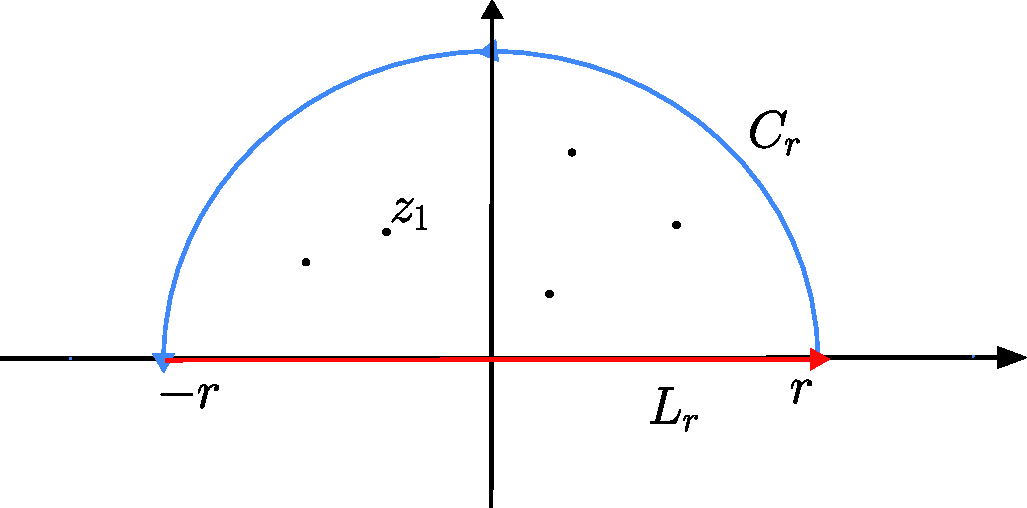
\includegraphics[width=0.6\textwidth]{figure/2026-04-04.pdf}
		\caption{Path $C_r + L_r$}
	\end{figure}
\begin{parag}{$ $}
    
	As we can see above, we can construct our two paths:
	\begin{align*} 
		L_r =  \left\{z \in \mathbb{C}: \text{Im } z = 0, -r \leq \text{Re } z \leq rz\right\}
	\end{align*}
	parametrized by $L_r\left(t\right) = t$, $t \in \left[-r, r\right]$
	\begin{align*} 
		C_r =  \left\{re^{i\theta}: \theta \in \left[0, \pi\right]\right\} 
	\end{align*}
	Now we can defined the whole path:
	\begin{align*} 
		\Gamma_r := L_R \bigcup C_r
	\end{align*}
	and the integral over this path:
	\begin{align*} 
		\int_{\Gamma_r}fdz =  \underbrace{\int_{L_r} fdz}_{= \int_r^{r}R\left(t\right)e^{iat}dt} + \int_{C_r}fdz
	\end{align*}
	As $r \to \infty$, one can compute $\int_{\Gamma_r}fdz$ by using the residue theorem: if $z_1, \ldots, z_k$ are zeros of $Q$ in the upper half of the plane (which are half of the total number of zeroes of $Q$) then:
	\begin{align*} 
		\int_{\Gamma_r}fdz =  2\pi i \left[\text{Res}_{z_1}\left(f\right) + \cdots + \text{Res}_{z_m}\left(f\right)\right]
	\end{align*}
	As $r \to \infty$ this goes to $\int_{-\infty}^{\infty}R\left(x\right)e^{iax}dx$.\\
	$ $\\
	It remains to show that $\int_{C_r}fdz \to 0$ as $r \to \infty$.
	\begin{itemize}
	    \item For $\text{Im }z \geq 0$ and $a \geq 0$, $\left|e^{iaz}\right| \leq 1$. Indeed, if we split $z$ as $z = x + iy$ we can see:
			\begin{align*} 
				\left|e^{ia(x + iy)}\right|= \left|e^{aix}e^{-ay}\right| = e^{-ay} \leq 1
			\end{align*}
	\end{itemize}
	\begin{subparag}{Remark}
		$\left|e^{ait}\right|$ is not bounded on all of $\mathbb{C}$, here it is because of the fact $i^2 < 0 \implies e^{\text{something } \leq 0} \leq 1$ But if $\text{Im }z < 0$ then with have a positive exponent to our number $\implies$ explodes
	\end{subparag}
	\begin{itemize}
	    \item $\left|R\left(z\right)\right|$ decays to 0 as $\left|z\right| \to \infty$
			\begin{align*} 
				\left|\int_{C_r}fdz\right| &=  \left|\int_0^{\pi}f\left(re^{i\theta}\right)ire^{i\theta}d\theta\right|\\
				&\leq \int_0^{\pi} \left|f\left(re^{i\theta}\right)\right| \left|rie^{i\theta}\right|d\theta\\
				&= \int_0^{\pi}\frac{\left|P\left(re^{i\theta}\right)\right|}{\left|Q\left(re^{i\theta}\right)\right|}\left|e^{iare^{i\theta}}\right|r d \theta
			\end{align*}
			The first inequality comes from the triangle inequality. Then using the same fact as on the first point, $\left|e^{iare^{i\theta}}\right| \leq 1$ since $\text{Im }\left(re^{i\theta}\right) \geq 0$ for $\theta \in \left[0, \pi\right]$
	\end{itemize}
	To see where the part involving $\frac{P}{Q}$ tends to, not if 
	\begin{align*} 
	\begin{rcases}
		P\left(z\right) = b_l z^{l} + b_{l-1}z^{l_1} + \cdots \\
		Q\left(z\right) = a_kz^{k} + a_{k-1}z^{k-1} + \cdots
	\end{rcases}
	\frac{P\left(z\right)}{Q\left(z\right)} = \frac{1}{z^{k-l}} \frac{b_l + \frac{b_{l-1}}{z} + \cdots}{ a_k + \frac{a_{k-1}}{z} + \cdots}
	\end{align*}
	Hence
	\begin{align*} 
		\left|\frac{P\left(re^{i\theta}\right)}{Q\left(re^{i\theta}\right)}\right| \leq \frac{\text{Const}}{r^{k-l}} \text{ for large } r
	\end{align*}
	And thus:
	\begin{align*} 
		\left|\int_{C_r}fdz\right| \leq \frac{\text{const} \pi}{r^{k-l}}r \to 0 \text{ as } r \to \infty
	\end{align*}
	
	In summary we deduce:
	\begin{align*} 
	\boxed{
		\int_{-\infty}^{\infty}R\left(x\right)e^{iax}dx =  2\pi i \left[\text{Res}_{z_1}\left(f\right) + \cdots + \text{Res}_{z_m}\left(f\right)  \right]
	} \end{align*}
	
	Where $z_1, \ldots, z_m$ are zeros of $Q$ in the upper half of the plane and $f\left(z\right) =  R\left(z\right)e^{iaz}$
	
	\begin{subparag}{Benefit}
	    One can compute the residues of $f$ by finding the poles of it and their orders, without computing Laurent series!
	\end{subparag}
\end{parag}
\begin{parag}{Example}
    We want to compute the integral:
	\begin{align*} 
		\int_{-\infty}^{\infty}\frac{x^2}{16 + x^{4}}\cos x dx
	\end{align*}
	This is of the shape form the previous example with $a= 1$, $P\left(x\right)= z^2$, $Q\left(x\right) = 1 + x^{4}$, Thus the integral coincides with:
	\begin{align*} 
		\int_{-\infty}^{\infty}\frac{x^2}{16 + x^{4}} \cos x dx = \text{Re} \left(\int_{-\infty}^{\infty}\frac{x^2}{16 + x^{4}}e^{ix}dx\right)
	\end{align*}
	The singularities of $f\left(z\right) = \frac{z^2}{16 + z^{4}}$ correspond to the complex root of $16 + z^{4} = 0 \implies r = 2, \theta =  \frac{\pi}{4} + k \frac{\pi}{2}$ where $k \in \left\{0, \ldots, 3\right\}$\\
	$ $\\
	Therefore we have our four singularities: 
	\begin{align*} 
		z_1 = \sqrt{2} + \sqrt{2}i
		z_2 = -\sqrt{2} + \sqrt{2}i
		z_3 =- \sqrt{2} - \sqrt{2}i
		z_4 = \sqrt{2} - \sqrt{2}i
	\end{align*}
	Hence we define $Q$ as 
	\begin{align*} 
		Q\left(z\right) =  \left(z - z_1\right)\left(z - z_2\right)\left(z - z_3\right)\left(z - z_4\right)
	\end{align*}
	So 
	\begin{align*} 
		R\left(z\right) = \frac{P\left(z\right)}{Q\left(z\right)} = \frac{z^2}{\left(z - z_1\right)\left(z - z_2\right)\left(z - z_3\right)\left(z - z_4\right)}
	\end{align*}
	Where each $z_i$ is a pole of order $1$.\\
	$ $\\
	Only the $z_i$ with an $\text{Im} \geq 0$ are relevant for the integral which implies that we only care for the Residue of $z_1$ and $z_2$:
	\begin{align*} 
		\text{Res}_{z_1}\left(f\right) =  \lim_{z \to z_1} \left(z-  z_1\right)f\left(z\right) =  \frac{e^{-\sqrt{2}}e^{\sqrt{2}i}}{4\sqrt{8}}\frac{1 + i}{i}\\
		\text{Res}_{z_2}\left(f\right) =  \lim_{z \to z_2} \left(z - z_2\right)f\left(z\right) = \frac{e^{-\sqrt{2}}e^{-\sqrt{2}i}}{4\sqrt{8}}\frac{1 - i}{i}
	\end{align*}
	Hence:
	\begin{align*} 
		\text{Re}\left(\int_{-\infty}^{\infty}R\left(x\right)e^{ix}dx\right) &=  \text{Re}\left(2\pi i \left(\text{Res}_{z_1}\left(f\right) + \text{Res}_{z_2}\left(f\right)\right)\right)\\
																			 &= 4\pi e ^{-\sqrt{2}}\left(\cos \sqrt{2} - \sin \sqrt{2}\right)
	\end{align*}
\end{parag}


\paragraph{Integrals of rational function of trigonometric functions}%
	\label{par:Integrals of rational function of trigonometric functions}$ $\\

	
    
	Suppose $P\left(x, y\right), Q\left(x, y\right)$ are polynomials and $Q$ is non-zero on the unit circle, i.e. $Q\left(x, y\right) \neq 0$ where $x^2 + y^2 = 1$ we want to compute:
	\begin{align*} 
		\int_{0}^{2\pi}\frac{P\left(\cos t, \sin t\right)}{Q\left(\cos t, \sin t\right)}dt
	\end{align*}
	We can re express this as a complex integral over the unit circle. Recall
	\begin{align*} 
		\cos t =  \frac{e^{it} + e^{-it}}{2}\\
		\sin t =  \frac{e^{it} - e^{-it}}{2i}
	\end{align*}
	We have:
	\begin{align*} 
		\int_0^{2\pi}\frac{P\left(\cos t, \sin t\right)}{Q\left(\cos t, \sin t\right)}dt &= \int_0^{2\pi}\frac{P\left(\frac{e^{it} + e^{-it}}{2}, \frac{e^{it} - e^{-it}}{2j}\right)}{Q\left(\frac{e^{it} + e^{-it}}{2}, \frac{e^{it} - e^{-it}}{2i}\right)}dt\\
		&= \int_0^{2\pi} \frac{Q\left(\cdots\right)}{Q\left(\cdots\right)}\frac{1}{ie^{it}}ie^{it}dt
	\end{align*}
	Now we can set 
	\begin{align*} 
		f\left(z\right) = \frac{P\left(\frac{z + \frac{1}{z}}{2}, \frac{z - \frac{1}{z}}{2i}\right)}{Q\left(\frac{z + \frac{1}{z}}{2}, \frac{z - \frac{1}{z}}{2i}\right)}\frac{1}{iz}
	\end{align*}
	Then the integral in question is equal to:
	\begin{align*} 
		\int_0^{2\pi} f\left(e^{it}\right)ie^{it}dt =  \int_{\gamma}fdz
	\end{align*}
	Where $\gamma : \left[0, 2\pi\right] \to \mathbb{C} \mathspace \gamma\left(t\right) =  e^{it}$ \\
	$ $\\
	Since $P, Q$ are polynomials,$f$ is holomorphic on $C \setminus \left\{z_1, \ldots, z_k\right\}$ where $z_1, \ldots, z_k$ are the point where the denominator vanishes
	\begin{parag}{$ $}
	    
	
	\begin{subparag}{Remark}
	    A function which is holomorphic except for isolated points is called \important{meromorphic}
	\end{subparag}
	\end{parag}
	If $z_1, \ldots, z_l$ are the points of $z_1, \ldots, z_k$ lying in the \important{interior of the unit circle}, the reside theorem implies:
	\begin{align*} 
	\boxed{
		\int_{0}^{2\pi}\frac{P\left(\cos t, \sin t\right)}{Q\left(\cos t, \sin t\right)} dt = 2\pi i \left[\text{Res}_{z_1}\left(f\right) + \cdots + \text{Res}_{z_l}\left(f\right)\right]}
	\end{align*}






\begin{parag}{Example}
    Let us now try to compute $\int_0^{2\pi} \frac{1}{2 \cos \theta}d \theta$. This falls into the previous example with $P\left(x, y\right) =  1$, $Q\left(x, y\right) =  2 + x$. Computing the function $f$ from the previous example explicitly yields
	\begin{align*} 
		f\left(z\right) = \frac{2}{i}\frac{1}{z^2 + 4z + 1}
	\end{align*}
	The singular points are on the zeros of $z^2 + 4z + 1$ which are $z_1 =  -2 + \sqrt{3}$ and $z_2 =  -2 - \sqrt{3}$. Only $z_1$ lies in the unit circle. Moreover $f$ has a pole of order $1$ at $z_1$. Hence 
	\begin{align*} 
		\text{Res}_{z_1}\left(f\right) =  \lim_{z \to z_1} \left(z - z_1\right)f\left(z\right) = \frac{1}{\sqrt{3}i}
	\end{align*}
	Consequently,
	\begin{align*} 
		\int_0^{2\pi} \frac{1}{2 + \cos \theta} d \theta =  2\pi i \text{Res}_{z_1}\left(f\right) =  \frac{2\pi }{\sqrt{3}}
	\end{align*}
\end{parag}

